\chapter{Linear Programming}

\section{Introduction}

\subsection{Linear Programming}

Linear programming is a method to achieve the best outcome in a mathematical model whose requirements are represented by linear relationships. It is a special case of mathematical programming (mathematical optimization).

\begin{example}[Brewery]
    A brewery can invest its inventory of corn, hops and malt into producing some amount of ale and some amount of beer.  Per unit resource requirement and profit of the two items are as given below.

    \begin{table}[ht!]
        \centering
        \begin{tabular}{|c|c|c|c|c|}
            \hline
            Beverage      & Corn (pounds) & Hops (ounces) & Malt (pounds) & Profit (\$) \\ \hline
            Ale (barrel)  & 5             & 4             & 35            & 13          \\ \hline
            Beer (barrel) & 15            & 4             & 20            & 23          \\ \hline
            constraint    & 480           & 160           & 1190          &             \\ \hline
        \end{tabular}
    \end{table}

    Suppose it produces $A$ units of ale and $B$ units of beer. Then, we want to solve this program:
    \[
        \begin{matrix}
                        & \color{blue} \text{Ale} &   & \color{blue} \text{Beer} &      &      &                            \\
            \max        & 13A                     & + & 23B                      &      &      & \color{blue} \text{Profit} \\
            \text{s.t.} & 5A                      & + & 15B                      & \leq & 480  & \color{blue} \text{Corn}   \\
                        & 4A                      & + & 4B                       & \leq & 160  & \color{blue} \text{Hops}   \\
                        & 35A                     & + & 20B                      & \leq & 1190 & \color{blue} \text{Malt}   \\
                        & A                       & , & B                        & \geq & 0    &                            \\
        \end{matrix}
    \]
\end{example}

\begin{definition}[Linear Function]
    $f: \R^n \to \R$ is a \term{linear function} if $f(x) = a^Tx$ for some $a \in \R^n$. 
\end{definition}

\begin{example}
    For example, \[
        f(x_1, x_2) = 3x_1 - 5x_2 = \begin{pmatrix} 3 & -5 \end{pmatrix}^T \begin{pmatrix} x_1 \\ x_2 \end{pmatrix}
    \] We can see that $a$ is the vector of coefficients of the linear function.
\end{example}

\begin{itemize}
    \item \textbf{Linear objective}: $f$
    \item \textbf{Linear constraints}:
    \begin{itemize}
        \item $g(x) = c$, where $g: \R^n \to \R$ is a linear function and $c \in \R$
        \item Line in the plane (or a hyperplane in higher dimensions $\R^n$)
    \end{itemize}
\end{itemize}

Geometrically, $a$ is the normal vector of the line(or hyperplane) represented by $a^Tx = c$.

\begin{figure}[ht!]
    \centering
    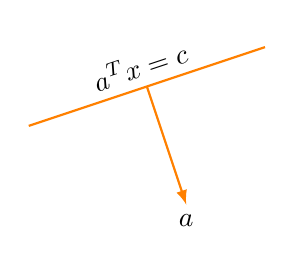
\begin{tikzpicture}[scale=0.5]
        \draw[thick,orange       ] (-3,-1) -- (3, 1) node[black,sloped,midway,above] {$a^Tx = c$};
        \draw[thick,orange,-latex] ( 0, 0) -- (1,-3) node[black,              below] {$a$};
    \end{tikzpicture}
\end{figure}

and $a^Tx \leq c$ is the \term{half-space} defined by the line.

\subsection{Finding the Optimal Solution}

\begin{example}
    Suppose we want to solve the following linear program: \[ \begin{matrix}
        \max        & x_1 & +    & 6x_2              \\
        \text{s.t.} & x_1 & \leq & 200               \\
                    & x_2 & \leq & 300               \\
                    & x_1 & +    & x_2  & \leq & 400 \\
                    & x_1 & ,    & x_2  & \geq & 0
    \end{matrix} \]

    This is equivalent to finding the \textbf{feasible region}, where ant point in the region satisfies all the constraints. The feasible region is the intersection of the half-spaces defined by the constraints.

    \begin{figure}[ht!]
        \centering

        \begin{subfigure}{0.45\linewidth}
            \centering
            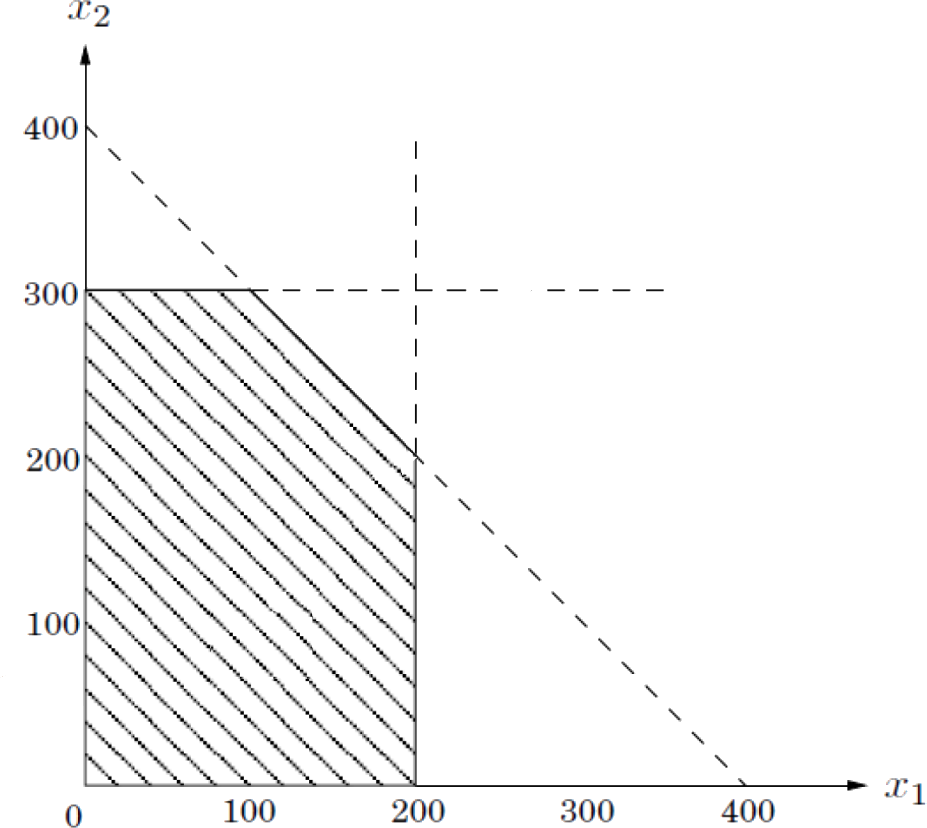
\includegraphics[width=\linewidth]{figures/feasible-region.png}
        \end{subfigure}
        \hfil%
        \begin{subfigure}{0.45\linewidth}
            \centering
            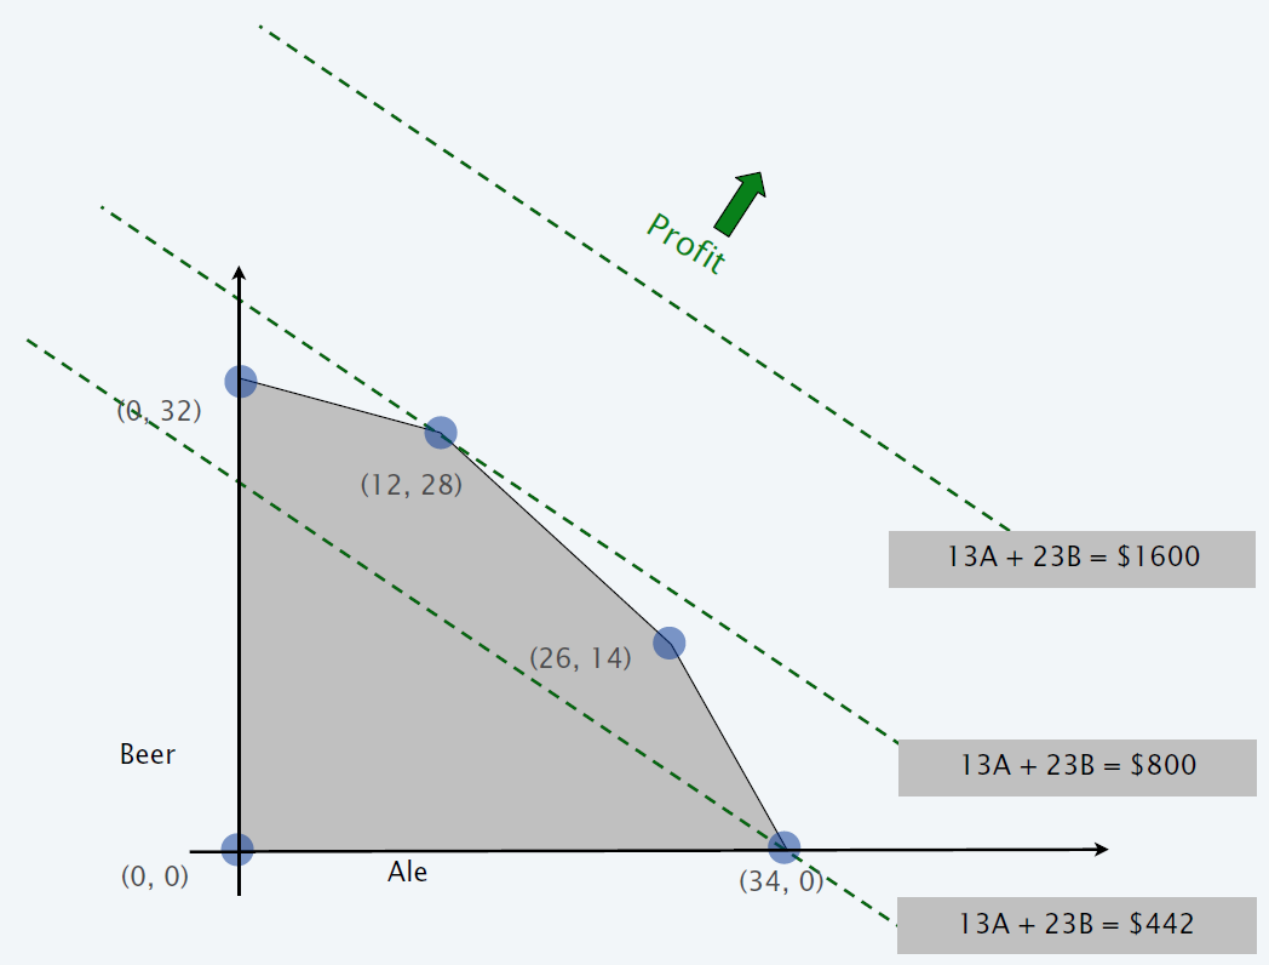
\includegraphics[width=\linewidth]{figures/opt-sol-at-a-vertex.png}
        \end{subfigure}
    \end{figure}
\end{example}

To find a maximum solution, we push the objective function as far as possible. 

\begin{claim}
    Regardless of the objective function, there must be a vertex that is an optimal solution
\end{claim}

\begin{remark}[Convexity]
    A \term{convex set} is a set $S$ cush that \[
        \forall x, y \in S, \lambda \in [0, 1] \implies \lambda x + (1 - \lambda)y \in S
    \]

    A \term{vertex of a convex set} is a point which cannot be written as a strict convex combination of any two points in the set.

    \begin{center}
        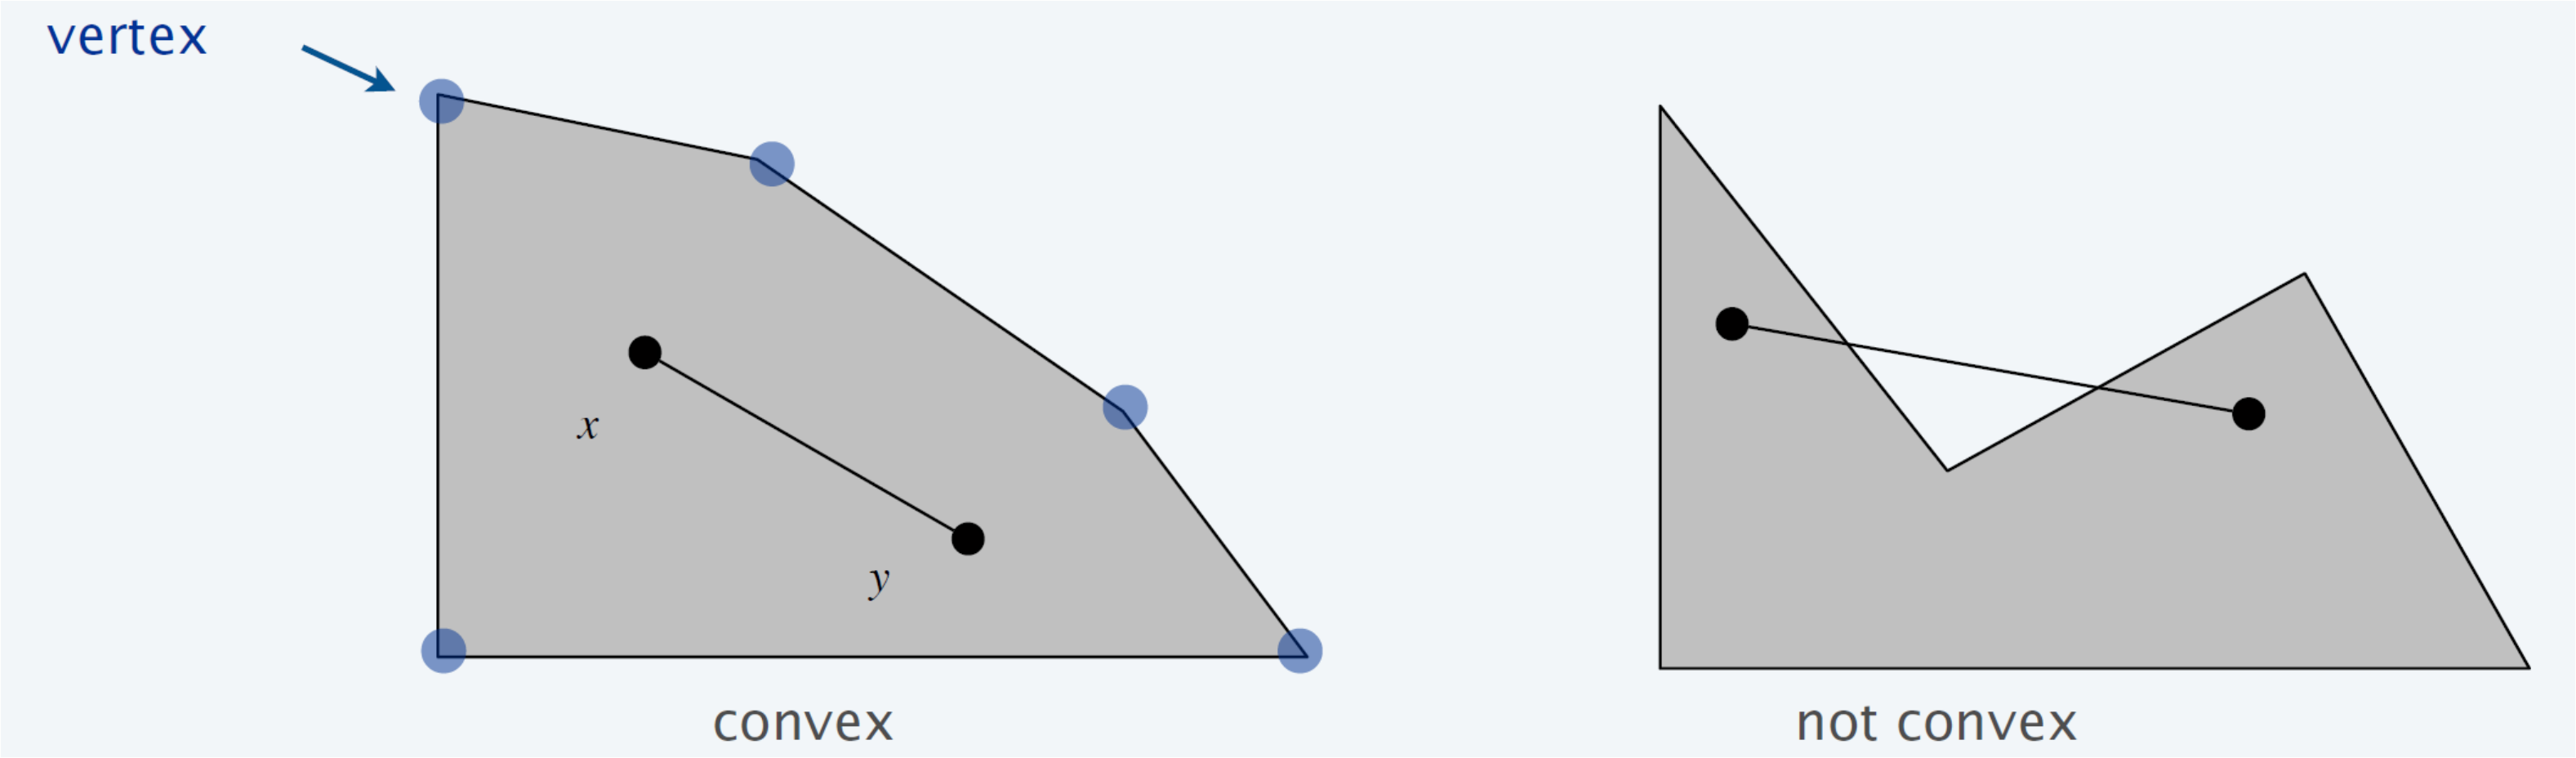
\includegraphics[width=\linewidth]{figures/convexity.png}
    \end{center}

    We observe that a feasible region of a linear program is a convex set.
\end{remark}

\begin{proof}[Intuitive Proof]
    We start at some point $x$ in the feasible region. 

    If $x$ is not a vertex, 
    \begin{itemize}
        \item Find d direction $d$ such that points within a positive distance of $\varepsilon$ from $x$ in both $d$ and $-d$ directions are within the feasible region
        \item Objective must \textit{not decrease} in at least one of the two directions
        \item Follow that direction until you reach a new point $x$ for which at least one more constraint is ``tight''
    \end{itemize}

    Repeat until we are at a vertex. 
\end{proof}

\section{Formatting Linear Programs}

\subsection{Standard Form}

\begin{itemize}
    \item \textbf{Input}: $c, a_1, a_2, \dots, a_m \in \R^n, b \in \R^m$.
    \item \textbf{Goal}: \[ \begin{matrix}
                  \text{Maximize}   & c^Tx      &        &     \\
                  \text{Subject to} & {a_1}^T x & \le    & b_1 \\
                                    & {a_2}^T x & \le    & b_2 \\
                                    &           & \vdots &     \\
                                    & {a_m}^T x & \le    & b_m \\
                                    & x         & \ge    & 0
              \end{matrix} \]
\end{itemize}

We can also combine all of them into a single \textbf{matrix equation}: \[ \begin{matrix}
    \text{Maximize}   & c^Tx &     &   \\
    \text{Subject to} & Ax   & \le & b \\
                      & x    & \ge & 0
\end{matrix} \]

\subsection{Converting to Standard Form}

\begin{itemize}
    \item Constraints that uses $\geq$: \[
        a^Tx \geq b \iff -a^Tx \leq -b
    \]

    \item Constraints that uses $=$: \[
        a^Tx = b \iff a^Tx \leq b, -a^Tx \leq -b
    \]

    \item Constraints that is a minimization: \[
        \text{Minimize } c^Tx \iff \text{Maximize } -c^Tx
    \]

    \item Variable is unconstrained: \[
        x_i \text{ is unconstrained} \iff x_i = x_i' - x_i'' \text{ where } x_i' \geq 0, x_i'' \geq 0
    \]
\end{itemize}

\begin{example}
    Consider the following example.
    \begin{align*}
        \begin{matrix}
            \text{minimize}   & -2x_1 & + & 3x_2            \\
            \text{subject to} & ~~x_1 & + & ~x_2 & =    & 7 \\
                              & ~~x_1 & - & 2x_2 & \leq & 4 \\
                              & ~~x_1 &   &      & \geq & 0
        \end{matrix} & \implies
        \begin{matrix}
            \color{red}\text{maximize} & \color{red} 2x_1 & \color{red}- & \color{red} 3x_2            \\
            \text{subject to}          &             ~x_1 & +            &             ~x_2 & =    & 7 \\
                                       &             ~x_1 & -            &             2x_2 & \leq & 4 \\
                                       &             ~x_1 &              &                  & \geq & 0
        \end{matrix} \\ & \implies
        \begin{matrix}
            \text{minimize}   & 2x_1 & -            & 3\color{red}x_2' & \color{red}+ & \color{red}3x_2''            \\
            \text{subject to} & x_1  & +            & \color{red}~x_2' & \color{red}- & \color{red}~x_2'' & =    & 7 \\
                              & x_1  & -            & 2\color{red}x_2' & \color{red}+ & \color{red}2x_2'' & \leq & 4 \\
                              & x_1  & \color{red}, & \color{red}~x_2' & \color{red}, & \color{red}~x_2'' & \geq & 0
        \end{matrix}
    \end{align*}
\end{example}

\subsection{Simplex Algorithm and Slack Form}

\begin{remark}
    Linear programming does not always have an optimal solution. It may ``fail'' for two reasons,
    \begin{enumerate}
        \item It is \textbf{infeasible}
        
        In other words, the feasible region is empty. That is, $\{ x | Ax \le b \} = \varnothing$. 
        
        \item It is \textbf{unbounded}
        
        In other words, the feasible region is unbounded, and the objective function can be made arbitrarily large (for maximization) or small (for minimization).
    \end{enumerate}
\end{remark}

\subsubsection{Simplex Algorithm}

\begin{algorithm}[ht!]
    \begin{algorithmic}[1]
        \Function{Simplex}{LP}
            \State $v \gets$ any vertex of the feasible region
            \While{there is a neighbour $v'$ of $v$ with better objective value}
                \State $v \gets v'$
            \EndWhile
            \State \Return $v$
        \EndFunction
    \end{algorithmic}
\end{algorithm}

\begin{itemize}
    \item Simple algorithm, easy to specify geometrically 
    \item Worst-case running time is exponential
    \item Excellent performance in practice
\end{itemize}

To implement the Simplex algorithm, we need to convert the linear program into \term{slack form}. which makes it convenient for implementing simplex operations.

In the slack form, we want to maximize $z$, but for now, we ignore the maximization objective. 

{~~~}

\begin{minipage}[t]{0.45\linewidth}
    \begin{center} \textbf{Standard form:} \end{center}
    \[ \begin{matrix}
        \text{Maximize}   & c^Tx &     &   \\
        \text{Subject to} & Ax   & \le & b \\
                          & x    & \ge & 0
    \end{matrix} \]
\end{minipage}
\hfil%
\begin{minipage}[t]{0.45\linewidth}
    \begin{center} \textbf{Slack form:} \end{center}
    \[ \begin{matrix}
        z    & =   & c^Tx   \\
        s    & =   & b - Ax \\
        s, x & \ge & 0
    \end{matrix} \]
\end{minipage}

\begin{example}
    Consider the following example. \[
        \begin{matrix}[rrcrcrcr]
            \text{maximize}   & 2x_1 & - & 3x_2 & + 3x_3 &      &      &    \\
            \text{subject to} & x_1  & + & x_2  & -      & x_3  & \leq & 7  \\
                              & -x_1 & - & x_2  & +      & x_3  & \leq & -7 \\
                              & x_1  & - & 2x_2 & +      & 2x_3 & \leq & 4  \\
                              & x_1  & , & x_2  & ,      & x_3  & \geq & 0
        \end{matrix}
    \]

    We first add the \textbf{basic variables} $x_4, x_5, x_6$ \footnote{$x_1, x_2, x_3$ are called \textbf{non-basic variables}.}, \[
        \begin{matrix}[rrcrcrcrcr]
            \text{maximize}   &     &   &        &   & 2x_1 & - & 3x_2 & + & 3x_3 \\
            \text{subject to} & x_4 & = & ~7     & - & ~x_1 & - & ~x_2 & + & ~x_3 \\
                              & x_5 & = & -7     & + & ~x_1 & + & ~x_2 & - & ~x_3 \\
                              & x_6 & = & ~4     & - & ~x_1 & + & 2x_2 & - & 2x_3 \\
                              & x_1 &   & \cdots &   & ~x_6 &   & \ge  &   & 0
        \end{matrix}
    \] which allows us to write the slack form as \[
        \begin{matrix}[rcrcrcrcr]
            z   & = &        &   & 2x_1 & - & 3x_2 & + & 3x_3 \\
            x_4 & = & 7~     & - & ~x_1 & - & ~x_2 & + & ~x_3 \\
            x_5 & = & -7     & + & ~x_1 & + & ~x_2 & - & ~x_3 \\
            x_6 & = & 4~     & - & ~x_1 & + & 2x_2 & - & 2x_3 \\
            x_1 &   & \cdots &   & ~x_6 &   & \ge  &   & 0
        \end{matrix}
    \]
\end{example}

\begin{enumerate}
    \item \textbf{Simplex: Step 1}
    
    We start at a feasible vertex.
    
    \begin{itemize}
        \item Fow now, assume $b \ge 0$ (that is, each $b_i \ge 0$).

        \item In this case, $Ax \le b$ is always satisfied by $x = 0$.

        \item In the slack form, this means setting the nonbasic variables to 0.
    \end{itemize}

    \item \textbf{Simplex: Step 2}

    \[ \color{primary} \begin{matrix}[rcrcrcrcr]
        x    & =    &      &      & 3x_1 & +    & x_2  & + & 2x_3 \\
        x_4  & =    & 30   & -    & x_1  & -    & x_2  & + & x_3  \\
        x_5  & =    & 24   & -    & 2x_1 & -    & 2x_2 & - & 2x_3 \\
        x_5  & =    & 36   & -    & 4x_1 & -    & x_2  & - & 2x^3 \\
        x_1, & x_2, & x_3, & x_4, & x_5, & x_ 6 & \ge  & 0 &
    \end{matrix} \]
    
    We increase the values of $z$. 

    \begin{itemize}
        \item Find a nonbasic variable with a positive coefficient in the objective function. This is called an \textbf{entering variable}.

        {\color{primary}Here, $x_1$ is the entering variable.}

        \item We determine how much we can increase its value without violating any constraints.

        {\color{primary}Here, $x_1$ can be increased to 9.}
    \end{itemize}

    We solve the tightest obstacle for the nonbasic variable. \[ \color{primary}
        x_1 = 9 - \frac{x_2}{4} - \frac{x_3}{2} - \frac{x_4}{4}
    \]

    \begin{itemize}
        \item Substitute the entering variable (called \term{pivot}) in other equations

        \item Now, $x_1$ becomes basic and $x_6$ becomes non-basic. 
        
        \item $x_6$ is called the \term{leaving variable}.
    \end{itemize} 
    \[ \color{primary} \begin{matrix}[rcrcrcrcr]
        z    & =    & 27   & +    & \frac{x_2}{4}  & +   & \frac{x_3}{2}  & - & \frac{3x_4}{4} \\
        x_1  & =    & 9    & -    & \frac{x_2}{4}  & -   & \frac{x_3}{2}  & - & \frac{x_4}{4}  \\
        x_4  & =    & 21   & -    & \frac{3x_2}{4} & -   & \frac{5x_3}{2} & + & \frac{x_6}{4}  \\
        x_5  & =    & 6    & -    & \frac{3x_2}{2} & -   & 4x_3           & + & \frac{x_6}{2}  \\
        x_1, & x_2, & x_3, & x_4, & x_5,           & x_6 & \ge            & 0 &
    \end{matrix} \]

    After one iteration of this step, the \textbf{basic feasible solution} (i.e. substituting $0$ for all nonbasic variables) improves from $z = 0$ to $z = 27$.

    \item \textbf{Simplex: Step 3}
    
    We repeat the process until there is no entering variable (nonbasic variable with a positive coefficient in the objective function).  

    \begin{itemize} \color{primary}
        \item Take $x_3$ as the entering variable, and the leaving variable is $x_5$.

          \[ \color{primary}
              \begin{matrix}[rcrcrcrcr]
                  z    & =    & 27   & +    & \frac{x_2}{4}  & +   & \frac{x_3}{2}  & - & \frac{3x_4}{4} \\
                  x_1  & =    & 9    & -    & \frac{x_2}{4}  & -   & \frac{x_3}{2}  & - & \frac{x_4}{4}  \\
                  x_4  & =    & 21   & -    & \frac{3x_2}{4} & -   & \frac{5x_3}{2} & + & \frac{x_6}{4}  \\
                  x_5  & =    & 6    & -    & \frac{3x_2}{2} & -   & 4x_3           & + & \frac{x_6}{2}  \\
                  x_1, & x_2, & x_3, & x_4, & x_5,           & x_6 & \ge            & 0 &
              \end{matrix} \implies
              \begin{matrix}[rcrcrcrcr]
                  z    & =    & \frac{111}{4} & +    & \frac{x_2}{16}  & -   & \frac{x_5}{8}  & - & 11\frac{x_6}{16} \\
                  x_1  & =    & \frac{33}{4}  & -    & \frac{x_2}{16}  & +   & \frac{x_5}{8}  & - & 5\frac{x_6}{16}  \\
                  x_3  & =    & \frac{3}{2}   & -    & 3\frac{x_2}{8}  & -   & \frac{x_5}{4}  & + & \frac{x_6}{8}    \\
                  x_4  & =    & \frac{69}{4}  & +    & 3\frac{x_2}{16} & +   & 5\frac{x_5}{8} & + & \frac{x_6}{16}   \\
                  x_1, & x_2, & x_3,          & x_4, & x_5,            & x_6 & \ge            & 0 &
              \end{matrix}
          \]

          \item Take $x_2$ as the entering variable, and the leaving variable is $x_3$.
          
          \[
                \begin{matrix}[rcrcrcrcr]
                    z    & =    & \frac{111}{4} & +    & \frac{x_2}{16}  & -   & \frac{x_5}{8}  & - & 11\frac{x_6}{16} \\
                    x_1  & =    & \frac{33}{4}  & -    & \frac{x_2}{16}  & +   & \frac{x_5}{8}  & - & 5\frac{x_6}{16}  \\
                    x_3  & =    & \frac{3}{2}   & -    & 3\frac{x_2}{8}  & -   & \frac{x_5}{4}  & + & \frac{x_6}{8}    \\
                    x_4  & =    & \frac{69}{4}  & +    & 3\frac{x_2}{16} & +   & 5\frac{x_5}{8} & + & \frac{x_6}{16}   \\
                    x_1, & x_2, & x_3,          & x_4, & x_5,            & x_6 & \ge            & 0 &
                \end{matrix} \implies
                \begin{matrix}[rcrcrcrcr]
                    z    & =    & 28   & -    & \frac{x_3}{6}  & -   & \frac{x_5}{6}  & 2\frac{x_6}{3} & \\
                    x_1  & =    & 8    & +    & \frac{x_3}{6}  & +   & \frac{x_5}{6}  & \frac{x_6}{3}  & \\
                    x_3  & =    & 4    & -    & 8\frac{x_3}{3} & -   & 2\frac{x_5}{3} & \frac{x_6}{3}  & \\
                    x_4  & =    & 18   & -    & \frac{x_3}{2}  & +   & \frac{x_5}{2}  &                & \\
                    x_1, & x_2, & x_3, & x_4, & x_5,           & x_6 & \ge            & 0              &
                \end{matrix}
          \]
    \end{itemize}

    \begin{itemize}
        \item Take the basic feasible solution. \[ \color{primary} x_3 = x_4 = x_5 = 0 \]
        \item Compute the optimal value of the objective function. \[ \color{primary} z = 28 \]
        \item Compute the optimal solution. \[ \color{primary} x_1 = 8, \quad x_2 = 4, \quad x_3 = 0 \]
    \end{itemize}
\end{enumerate}

\subsubsection{Unboundiness and Degeneracy}

\begin{itemize}
    \item Entering variable has no upper bound.
    
    If it doesn't appear in any constraints, or only appears in constraints where it can go to $\infty$, then $z$ can also go to $\infty$, and we declare that the linear program is \term{unbounded}.

    \item Pivoting does not change the constraint in $z$. 
    
    This is known as \term{degeneracy}, and can lead to infinite loops. Degeneracy can be prevented by ``perturbing'' $b$ by a small random number in each coordinate, or by carefully breaking ties among entering and leaving variables (for exampke, by choosing the leaving variable with the smallest index, which is called \term{Bland's rule}).
\end{itemize}

% TODO: When $b < 0$

\subsubsection{Running Time}

\begin{itemize}
    \item The number of vertices of a polytope can be exponential in the number of constraints.

    \begin{itemize}
        \item There are examples where simplex takes exponential time if you choose your pivots arbitrarily.
        \item No pivot rule known which guarantees polynomial running time
    \end{itemize}

    \item Other algorithms known which run in polynomial time
    \begin{itemize}
        \item Elliot's method, interior point method, etc.
        \item Ellipsoid uses $\mathcal{O}(mn^3L)$ arithmetic operations, where $L$ is the number of bits in the input
        \item But no known \textit{strongly polynomial time} algorithm. 
        \begin{itemize}
            \item Number of arithmetic operations should be polynomial in the size of the input
            \item We known how to avoid dependence on $\text{length}(b)$, but not for $\text{length}(A)$
        \end{itemize}
    \end{itemize}
\end{itemize}